\newcommand{\institut}{Institut f\"ur Telekommunikationssysteme}
\newcommand{\fachgebiet}{Nachrichten\"ubertragung}
\newcommand{\veranstaltung}{Praktikum Nachrichten\"ubertragung}
\newcommand{\pdfautor}{Dirk Babendererde (321 836), Thomas Kapa (325 219)}
\newcommand{\autor}{Dirk Babendererde (321 836)\\ Thomas Kapa (325 219)}
\newcommand{\gruppe}{Gruppe:}
\newcommand{\betreuer}{Betreuer: Lieven Lange}


\newcommand{\pdftitle}{Nachrichtenuebertragung\ Praktikum\ 06}
\newcommand{\prototitle}{Praktikum 06 \\ Digitale Übertragungstechnik: Digitale Empf\"anger}

\input{../../packages/tu_header_9}

% damit das outline funktioniert noch mal:
\begin{document}


%     \lstinputlisting{./praktikum6.sce}

%---------------------------------------------------------------------
%---------------------------------------------------------------------
%---------------------------------------------------------------------

\section{Vorbereitung}
\begin{quote}
       In diesem Praktikum wird die sogenannte Wasserfallkurve betrachtet. Dabei wird die Bitfehlerwahrscheinlichkeit
       über dem SNR geplottet. Bei der Übertragung von Signalen über einen nicht idealen Kanal wird das Signal mit
       Rauschen überlagert. Diese Tatsache kann auf der Empfängerseite zu dem Problem führen, dass der Entscheider sich
       statt einer 0 für eine 1, oder umgekehrt, entscheidet. Um die Wasserfallkurve zu ermitteln, wird die
       Intensität des Rauschens variiert und die Bitfehlerwahrscheinlichkeit gemessen.
       Da das SNR mit Hilfe des Logarithmus berechnet wird, wird ein Ansteigen hin zu den negativen SNR Werten (also da wo die Rauschenleistung größer ist als die Signalleistung, Faktor kleiner null und damit Logarithmus
       negativ) erwartet. \\
       Die Ergebnisse der Simulation der Wasserfallkurven ist in Abb. \ref{fig:simu_Wasser} zu sehen.
  
       \begin{figure}[H]
        \centering
        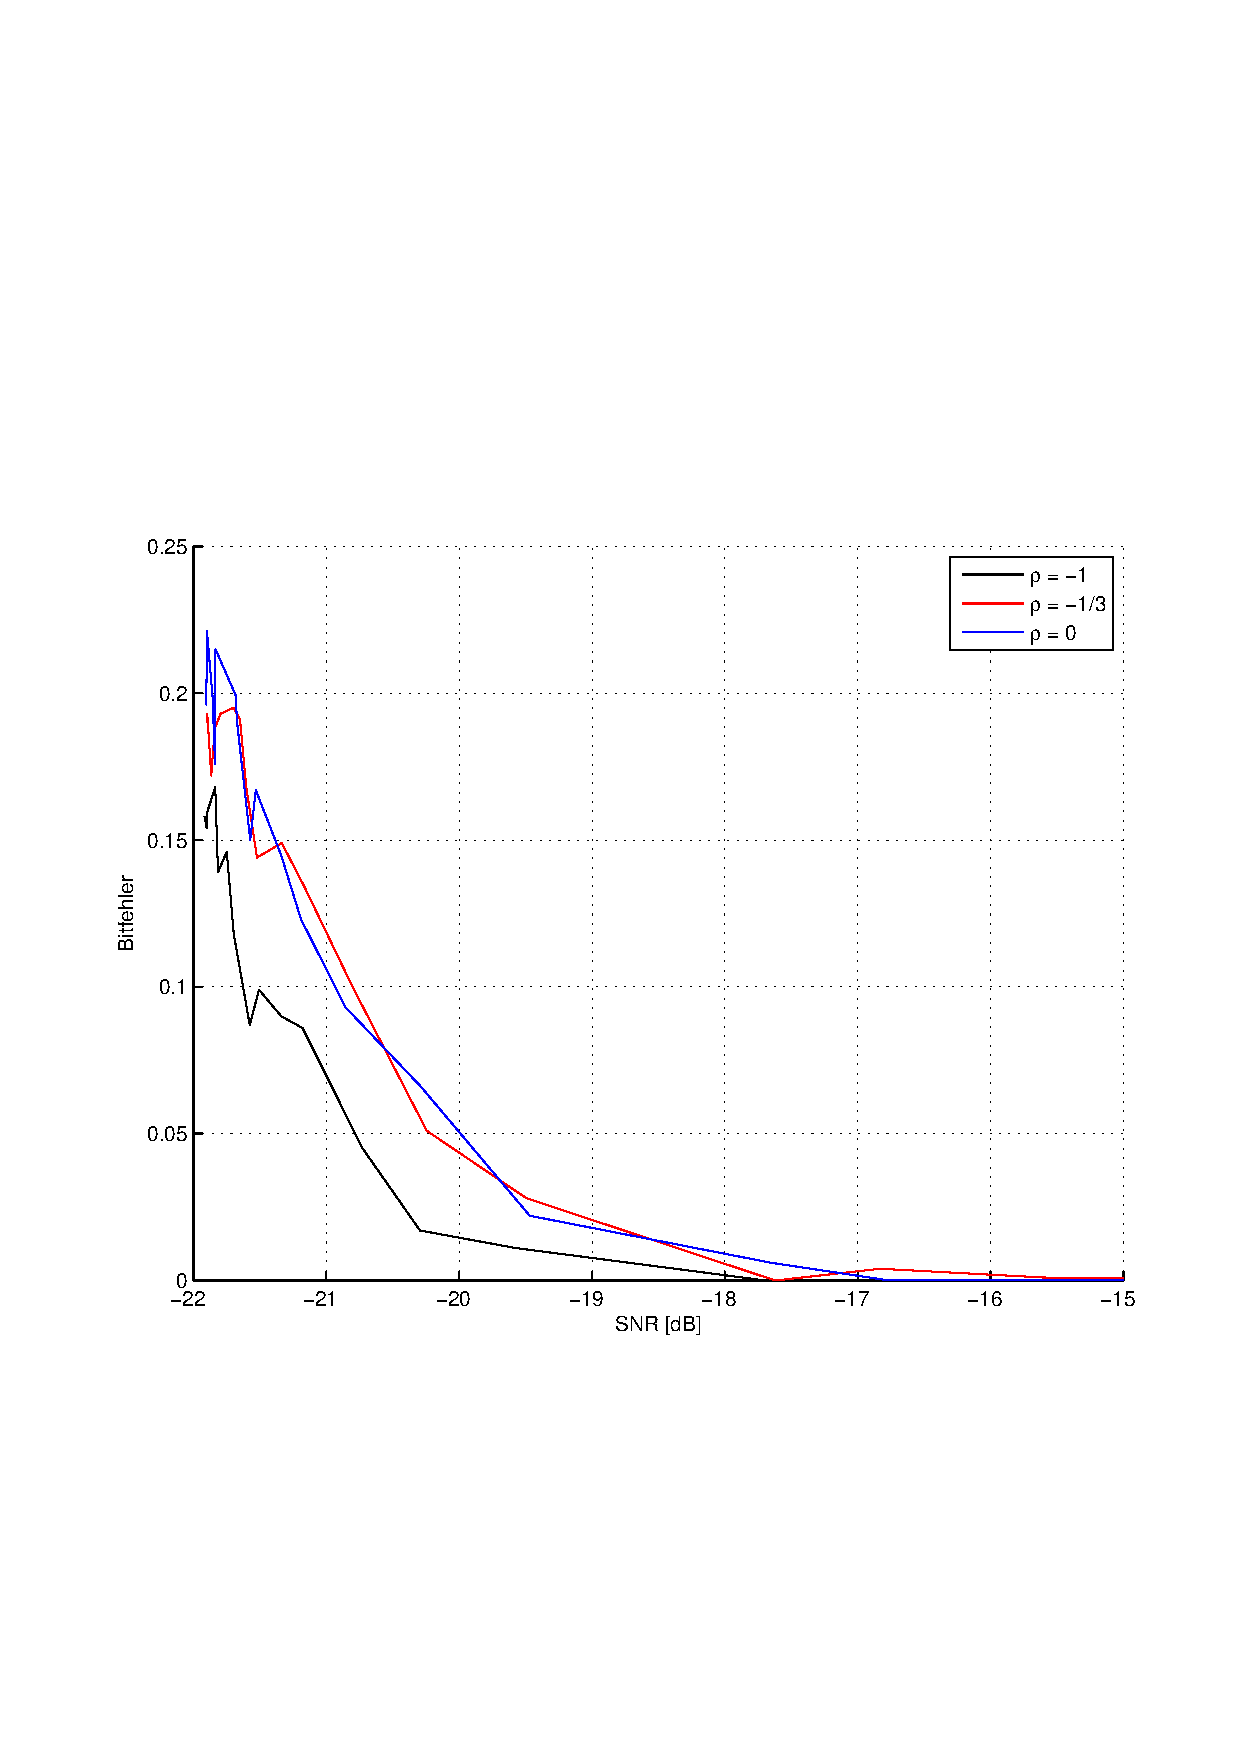
\includegraphics[scale=0.7, trim = 2cm 7cm 1cm 8cm, clip]{Bilder/Simulation_Wasserfall}
          \caption{simulierte Wasserfallkurven}
        \label{fig:simu_Wasser}
       \end{figure}
       
       \vspace{2em}
  
  
    \begin{equation}
	     \begin{split}
		\rho_{01}=\frac{1}{E_{b}} \int\limits_{0}^{T_{Bit}}  s_{0}(t) \cdot s_{1}(t)  \ dt
           \footnotemark
	     \end{split}
    \end{equation} 
     \label{eq:rho01}
    \footnotetext{Prof. Dr.-Ing. Sikora, Thomas, Foliensatz 10 Binäre Basisbandübertragung, Einführung in die
           Nachrichtenübertragung, S.159} 
    
    \begin{equation}
	     \begin{split}
		SNR_{E}=\frac{4E_{b}}{N_{0}}(1-\rho_{01})
           \footnotemark
	     \end{split}
    \end{equation}  
     \label{eq:SNR}
    \footnotetext{Prof. Dr.-Ing. Sikora, Thomas, Foliensatz 10 Binäre Basisbandübertragung, Einführung in die
           Nachrichtenübertragung, S.160}
           
    Theoretisch würde man also wegen des Faktors $(1-\rho_{01})$ für $\rho_{01}=0$ in Formel \ref{eq:SNR} das kleinste
    SNR und damit den höchsten Bitfehler erwarten. Dies ist in Abb.   \ref{fig:simu_Wasser} aber kaum zu sehen.
    $\rho_{01}=0$ und $\rho_{01}=-1/3$ liegen nahezu aufeinander. Dies erklärt sich durch die höhere Bitenergie. Da für die
    Sendeform bei $\rho_{01}=0$ 4 Baud nötig sind (4 Baud heißt in diesem Fall ein Bit besteht aus vier Zeichen,
    entweder -1 oder 1), ergibt sich nach Formel \ref{eq:E_b} ein $E_{b}$ von 4 statt von 3 für $\rho_{01} = -1/3$ und
    $\rho_{01}= -1$. Das $E_{b}$ verbessert wiederum das SNR in Formel \ref{eq:SNR} und damit verringert es auch die
    Bitfehlerwahrscheinlichkeit. Damit ist das Ergebnis plausibel und wie erwartet. 
    
    \begin{equation}
        \begin{split}
            E_{b}= \int\limits_{-\infty}^{\infty} s(t)^2 \ dt
        \end{split}
        \footnotemark
    \end{equation}  
    \label{eq:E_b}
    \footnotetext{Prof. Dr.-Ing. Sikora, Thomas, Foliensatz 10 Binäre Basisbandübertragung, Einführung in die
           Nachrichtenübertragung, S.129}
    
    \begin{equation}
	     \begin{split}
		p_{Bit}=\frac{1}{2}erfc  \sqrt{\frac{E_{b}}{2N_{0}(1-\rho_{01})}}
           \footnotemark
	     \end{split}
    \end{equation}  
	 \label{eq:p_bit}
    \footnotetext{Prof. Dr.-Ing. Sikora, Thomas, Foliensatz 10 Binäre Basisbandübertragung, Einführung in die
           Nachrichtenübertragung, S.161}
        
	An Formel \ref{eq:p_bit} kann man zusätzlich erkennen, dass die Signalform bei der Übertragung mit SAF, also ob z. B.
	Rechteck, Dreieck, oder Cosinus keinen Einfluss auf die Bitfehlerwahrscheinlichkeit hat.
    
    
\end{quote}


\section{Labordurchführung}
\begin{quote}
    
    
    \subsection{Encoderkennlinie}
    \begin{quote}
        
        Um die Bitfehlerrate messen zu können, werden die D/A-Box, das PCM-DECODER-Modul, die ADDER-Module, das
        Picoscope und der NOISE GENERATOR benötigt.\\
       Der oberste Ausgang (rot) der D/A-Box, der das Datensignal enthält, wird auf das erste ADDER-Modul gegeben, dass
       keine Verstärkungsmöglichkeit enthält und mit einem Offset aus dem VARIABLE DC-Modul addiert. Anschließend wird
       das Ergebnis auf das zweite ADDER-Modul geführt, wo es mit dem Verstärkungsregler auf eine Amlitude von -1..1
       gedämpft wird.\\
       Der 3. Ausgang von unten der D/A-Box (gelb) enthält die PCM codierten Datenworte. Diese werden auf den Eingang
       PCM DATA des PCM DECODER-Moduls gegeben.\\
       Der 2. Ausgang von unten enthält das Rahmensignal, welches mit dem Gegenstück des PCM-DECODER-Moduls verbunden
       wird.\\
       Der unterste Ausgang (blau) gibt das Clock Signal aus. Dieses wird mit einem T-Stück zum einen an den Eingang B
       des Picoscope und zum anderen an den CLK Eingang des PCM DECODER-Moduls des Picoscope geschlossen.\\
       Zuletzt wird der OUTPUT des PCM-Decoder Moduls (Spannung des Faktors zur Verstärkung bzw. Dämpfung des
       Rauschens) auf einen Multiplizierer gegeben und mit -6 dB multipliziert. Der Ausgang des Multiplizierers wird auf den
       zweiten Eingang des zweiten ADDER-Moduls gegeben.\\
       Der Ausgang dieses ADDER-Moduls wird auf den A Eingang des Picoscopes gegeben.
       Der Kanal und die Empfängerseite sind im Blockschaltbild \ref{fig:Kanal_pl_SAF} zu sehen.
       
       
    \begin{figure}[H]
        \centering
        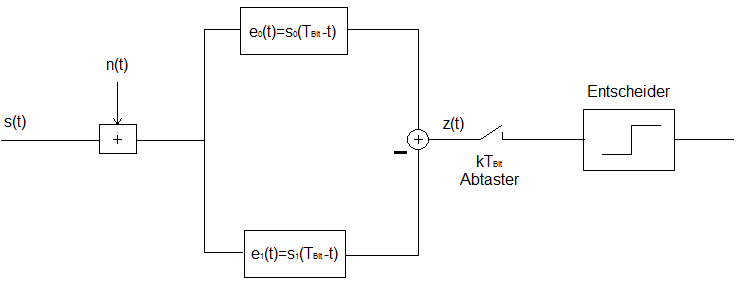
\includegraphics[scale=0.7]{Bilder/SAF-Filter}
        \caption{Kanal plus SAF}
        \label{fig:Kanal_pl_SAF}
    \end{figure}
     
    \end{quote}
    
   
\end{quote}

\section{Auswertung \& Theorie}
\begin{quote}
    
    \subsection{Wasserfallkurve}
    
    \begin{quote}
    
    	\begin{figure}[H]
          \centering
           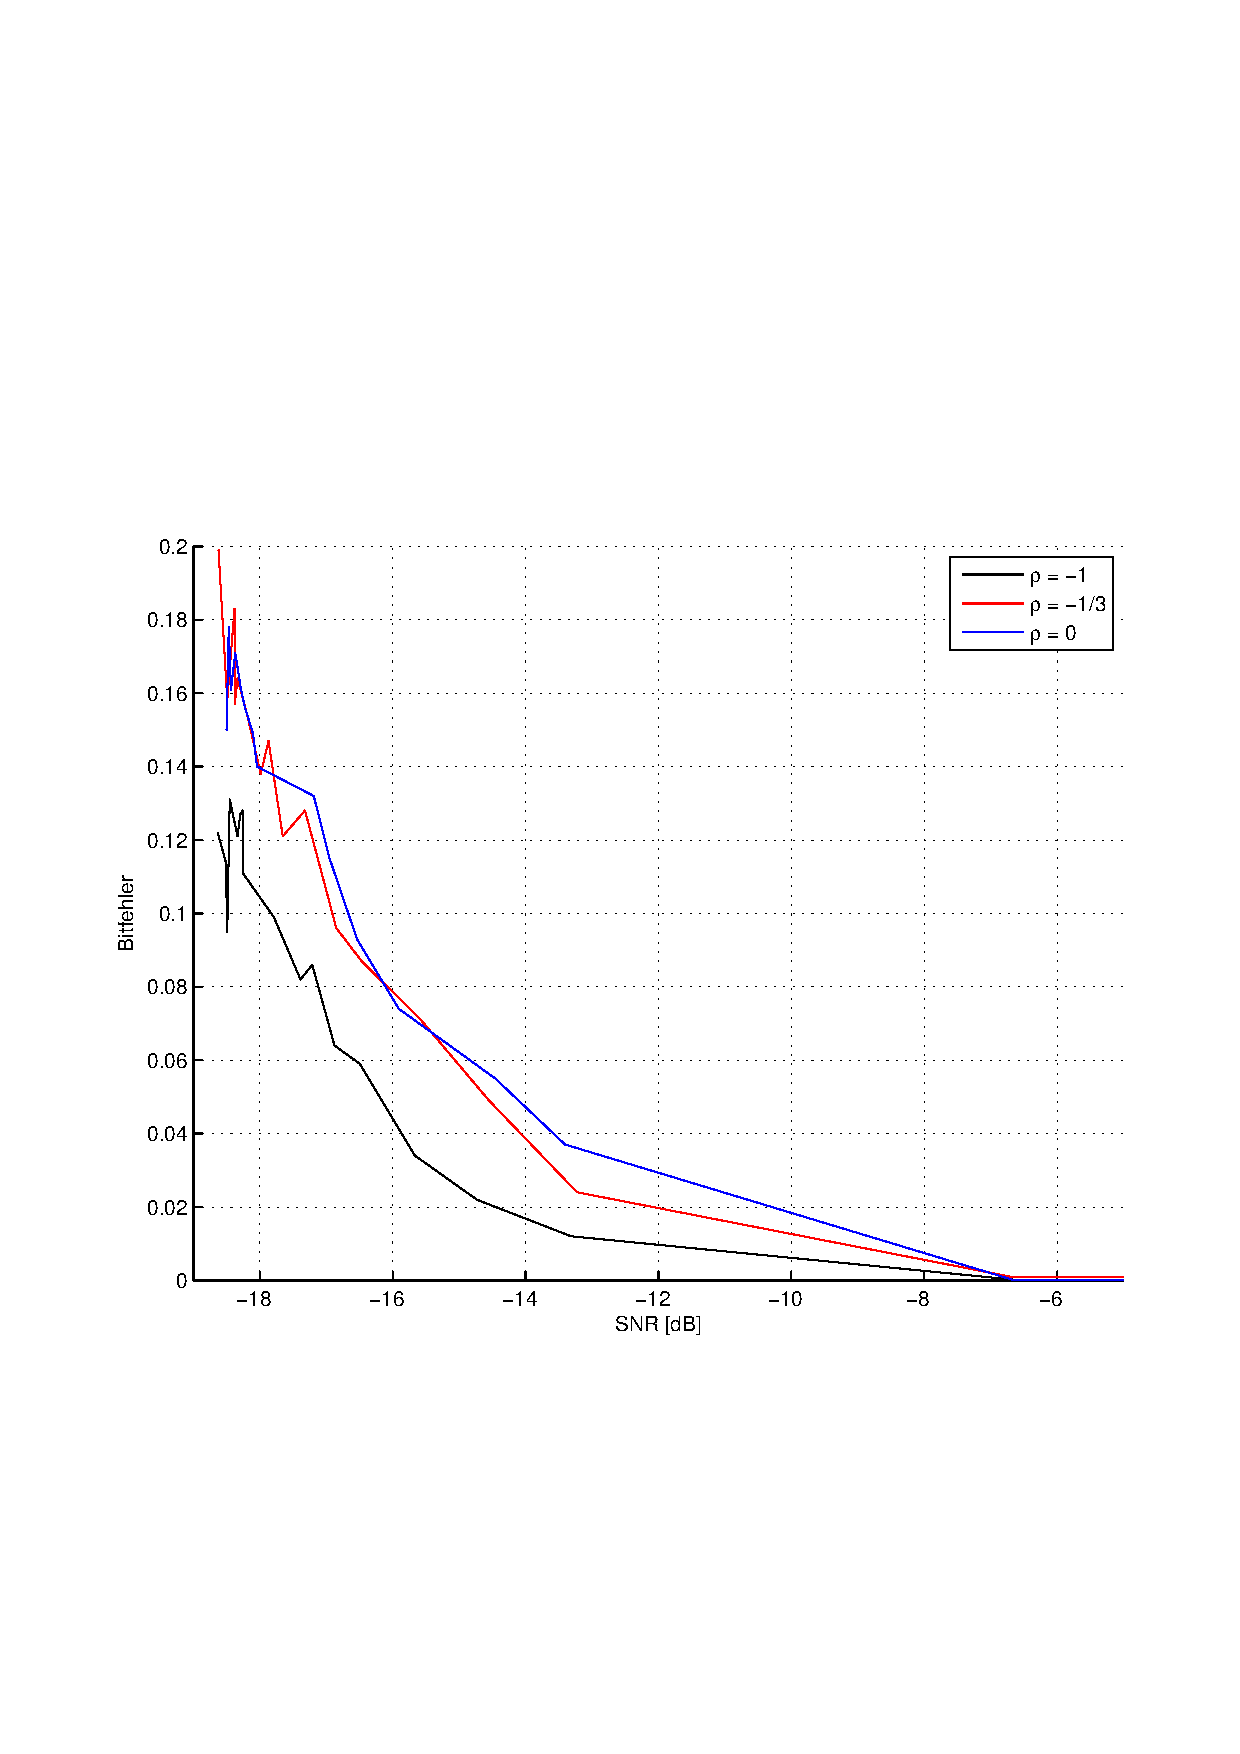
\includegraphics[scale=0.7, trim = 2cm 7cm 1cm 8cm, clip]{Bilder/Gemessen_Wasserfall}
            \caption{gemessene Wasserfallkurven}
          \label{fig:gemess_Wasser}
        \end{figure}
       
       \vspace{2em}    
    
    Die gemessenen Wasserfallkurven sind mit den simulierten nahezu identisch. Der selbe Effekt, der schon in den
    Vorbereitungsaufgaben erklärt wurde, tritt hier wieder auf.\\
    In beiden Fällen treten Bitfehler größer null erst für ein SNR kleiner null auf, dass heißt
    wenn die Rauschleistung größer als die Signalleistung wird. Auffällig ist allerdings, dass der Anstieg der
    durchschnittlichen Bitfehler in der Simulation erst deutlich später beginnt, als bei den gemessenen Werten.
    \TODO{Der Kanal in der Simulation ist also weniger störanfällig.\\}
    Der Bitfehler zeigt für kleiner werdendes SNR einen exponentiellen Anstieg, muss Theoretisch aber bei 1 sein Maximum
    erreicht haben, wenn alle Bits fehlerhaft übertragen wurden.
    
    \end{quote}
     
\end{quote}

\section{Zusammenfassung}
\begin{quote}
	
	Es hat sich in diesem Versuch gezeigt, dass die Bitfehlerwahrscheinlichkeit bei der Übertragung mit Hilfe eines SAF
	deutlich von der Sendeform abhängt. Dabei ist eine Sendeform mit einer normierten Kreuzkorrelation zwischen den
	Sendeimpulsen von -1 zu bevorzugen. Interessant ist hingegen, dass bei der Übertragung mit speziellen Sendeformen die
	Signalform auf die Bitfehlerwahrscheinlichkeit keinen Einfluss hat.\\
	Mit Hilfe von Wasserfallkurven lassen sich also Übertragungskanäle in Bezug auf ihre Fehleranfälligkeit
	charakterisieren.
 
    
\end{quote} % end Sec: section



\newpage

\begin{thebibliography}{999}

% \bibitem{Boris}Boris Henckell: Ein Paar sachen geklaut.. ähhh inspirationen geholt
% \href{http://www.krachler.com/fileadmin/user_upload/arbeiten/Reglersynthese_Christian_Krachler.pdf}{Reglersynthese nach dem Frequenzkennlinienverfahren}, S16, S22, 08.05.2012


% Name, Vorname.; evtl. Name2, Vorname2.: Titel des Dokumentes
% oder Buches, Zeitschrift/Verlag/URL (Auflage, Erscheinungsort, -jahr), ggf. Seitenzahlen
%\bibitem [Wiki10] {DigitaleMesskette2} \url{www.wikipedia.org}, Zugriff 22.03.2010

\bibitem [1]{Prakt_NUE_06} Prof. Dr.-Ing. Sikora, Thomas; Prof. Dr.-Ing. Noll, Peter: Einführung in die
Nachrichtenübertragung, 2010
\bibitem [2]{Prakt_NUE_06} Dipl.-Ing. Tok, Michael/Esche,Marko, M.Sc./Dr.-Ing. Krutz, Andreas: Unterlagen zum Praktikum
Nachrichtenübertragung (SS 2012), Termin 6
\end{thebibliography}

\end{document}
